\documentclass{sciposter}
\usepackage{lipsum}
\usepackage{epsfig}
\usepackage{amsmath}
\usepackage{amssymb}
\usepackage{multicol}
\usepackage{graphics,url}
\usepackage[portuges, brazil]{babel}   
\usepackage[utf8]{inputenc}
\usepackage{listings}  
%\usepackage{fancybullets}
\newtheorem{Def}{Definition}


\title{ Dias de Escola}
%Título do projeto

\author{Davi S. Meneses, Jennifer Cintra P. Silva, Jesley Silva de Oliveira, Raldney Sampaio Alves}
%nome dos autores

\institute 
{Bacharelado em Ciência da Computação\\
Centro Universitário SENAC - Campus Santo Amaro
  (SENAC-SP)\\
  Av. Engenheiro Eusébio Stevaux, 823 -- Santo Amaro, São Paulo -- CEP 04696-000 -- SP -- Brasil}
%Nome e endereço da Instituição

\email{\normalsize davismeneses,raldney{\_}sampaio{(@hotmail.com)},jennifer.cintra.03@gmail.com,dhiesleyolivera@yahoo.com.br}
% Onde você coloca os emails dos integrantes


%\date is unused by the current \maketitle

\rightlogo[1]{Senac-logo}
\leftlogo[1]{Ecomp-logo}
% Exibe os logos (direita e esquerda) 
% Procure usar arquivos png ou jpg, e de preferencia mantenha na mesma pasta do .tex
%%%%%%%%%%%%%%%%%%%%%%%%%%%%%%%%%%%%%%%%%%%%%%%%%%%%%%%%%%%%%%%%%%%%%%%%%%%%%%%%
%%% Begin of Document



\begin{document}
%define conference poster is presented at (appears as footer)

\conference{{\bf E-COMP 2013}, 5º Encontro da Computação - Senac, 27 de Novembro de 2013, São Paulo, Brasil}

%\LEFTSIDEfootlogo  
% Uncomment to put footer logo on left side, and 
% conference name on right side of footer

% Some examples of caption control (remove % to check result)

%\renewcommand{\algorithmname}{Algoritme} % for Dutch

%\renewcommand{\mastercapstartstyle}[1]{\textit{\textbf{#1}}}
%\renewcommand{\algcapstartstyle}[1]{\textsc{\textbf{#1}}}
%\renewcommand{\algcapbodystyle}{\bfseries}
%\renewcommand{\thealgorithm}{\Roman{algorithm}}

\maketitle

%%% Begin of Multicols-Enviroment
\begin{multicols}{2}

%%% Abstract
\section{Resumo}
 
Com a gamificação, as crianças estão cada vez mais distantes dos estudos comuns e aprendendo de maneira indireta em jogos usados em sua distração e diversão. Assim, o objetivo desse projeto foi o desenvolvimento de um jogo para que as crianças pudessem aprender e se divertir. Para os professores esse jogo seria um material de apoio para suas aulas, garantindo que os alunos reforcem aquilo que está sendo ensinado. A tecnologia empregada em jogos pode ser usada a favor da educação. Desse modo a criação do jogo \textbf{Dias de Escola} tem como foco a matéria de Ciências, motivado pela dificuldade que os alunos encontram no estudo da mesma. 

 

%%% Introduction
\section{Introducão}
Devido ao avanço tecnológico, os meios digitais tornaram-se meios mais eficazes para auxiliar o aprendizado devido ao grande acúmulo e facilidade de acesso às informações. Com isso o desenvolvimento do \textbf{Dias de Escola} foi focado na matéria de Ciências, pois possui uma grande área de aplicação tornando-se um jogo para quem procura novos meios de estudo complementar.

\newline
\section{Objetivos}

O objetivo desse projeto foi desenvolver um ambiente educacional para jovens que estão cursando o Fundamental II, tornando a escolha da plataforma e design um fator importante, causando motivação e maior interesse na busca de novos conhecimentos.
Baseado em uma jogabilidade simples e direta, o teclado dá ao usuário o controle total sobre o jogo, possibilitando assim uma melhor interação entre eles.
As questões são abordadas de modo informal e divetido, mudando assim a modo tradicional de apresentá-las. Conforme as questões são respondidas, uma pontuação e um ranking são gerados.

\newline
\section{Metodologia}

O jogo foi desenvolvido em Linguagem C versão 99 e com a biblioteca Allegro 5. Para o desenvolvimento gráfico foi utilizado o RPGMaker junto com ferramentas de edição de imagens, tornando o jogo mais atraente, conforme a figura 1. Devido a utilização da linguagem C, a codificação do jogo ficou mais robusta e junto com o Allegro 5 foi possível transformar o jogo em algo mais atraente. A utilização dessa linguagem possibilitou o acesso para os que querem conhecer um pouco mais sobre o mundo dos jogos.
\newline

\begin{figure}[!htb]
     \centering
     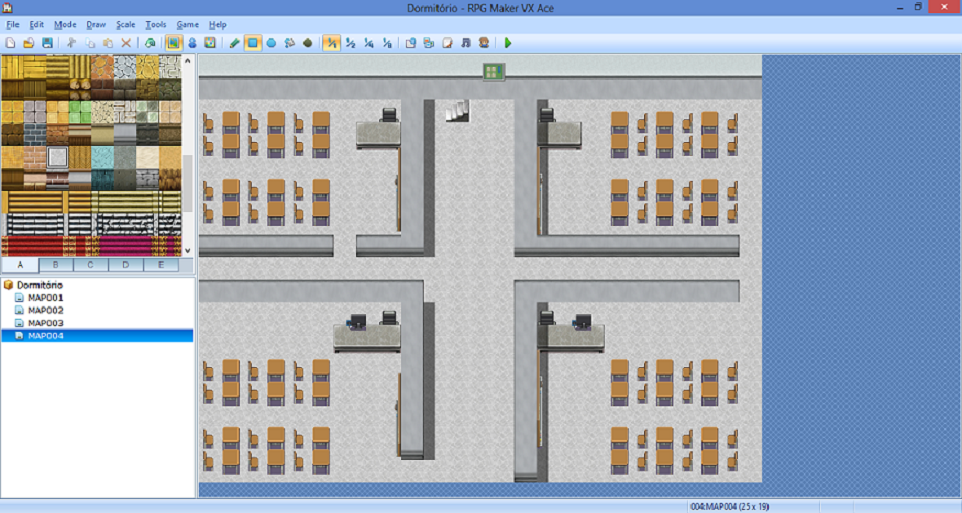
\includegraphics{rpg.png}
     \caption{Cenário feito no RPG Maker.}
\end{figure}
\centerline{Personagens Principais}
Peter/Sabrina é um/uma jovem com dificuldade no aprendizado de Ciências e seus pais, aceitando a proposta do filho/a matriculá-lo/la para um Internato, o melhor do País, onde ensinam Ciências muito bem. Para Peter/Sabrina essa mudança de escola é um grande desafio, ao qual eles aceitam de bom grado, começando assim seu ano na nova escola. 
\begin{figure}[!htb]
     \centering
     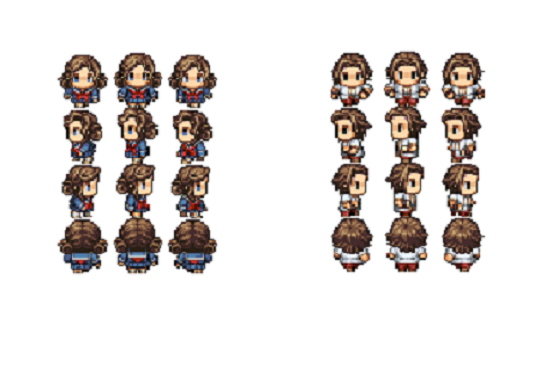
\includegraphics{personagens.png}
     \caption{Peter e Sabrina.}
\end{figure}
\begin{figure}[!htb]
     \centering
     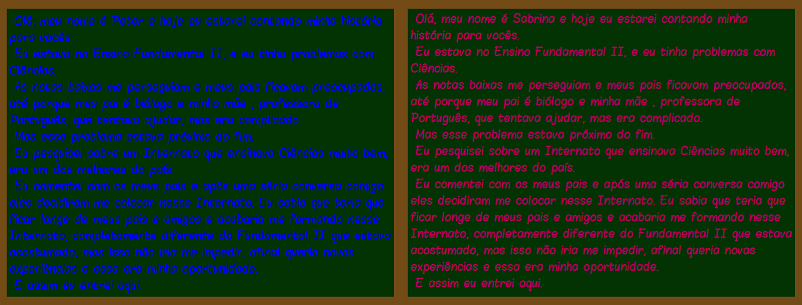
\includegraphics{hist.png}
     \caption{História dos personagens.}
\end{figure}
\newline
\newline
\newline
\section{Resultados e Discussão}
A colisão é a movimentação do pesonagem evitando a passagem dele pelos objetos no cenário do jogo.
\begin{lstlisting}
void carregarColisao(int nMapa)
{
    i=0;
    j=0;
    fMapa = fopen(colisaoMapa[nMapa], "r"); 
    printf("teste\n");
		while((lerMapa = getc(fMapa) ) != EOF )
    {
        if ( i < 27 )
        {
            tileMap[j][i] = atoi(&lerMapa); 
            i++;
        }
        else 
        {
            j++;
            i=0;
        }
    }
    fclose(fMapa);
}    
\end{lstlisting}
\newline
\newline
\begin{figure}[!htb]
     \centering
     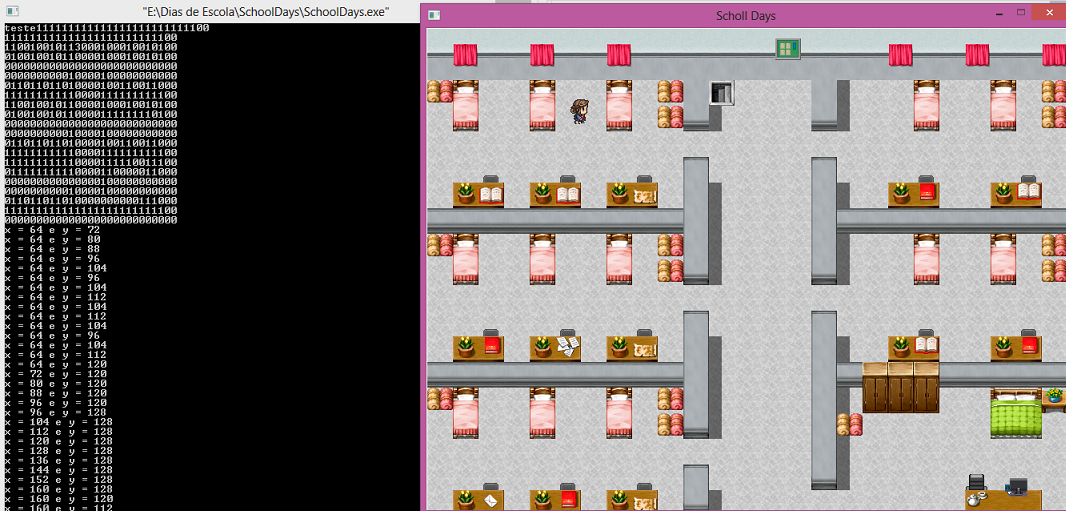
\includegraphics{colisao.png}
     \caption{Movimento realizado pelo personagem no cenário e suas coordenadas ao lado.}
\end{figure}

\begin{figure}[!htb]
     \centering
     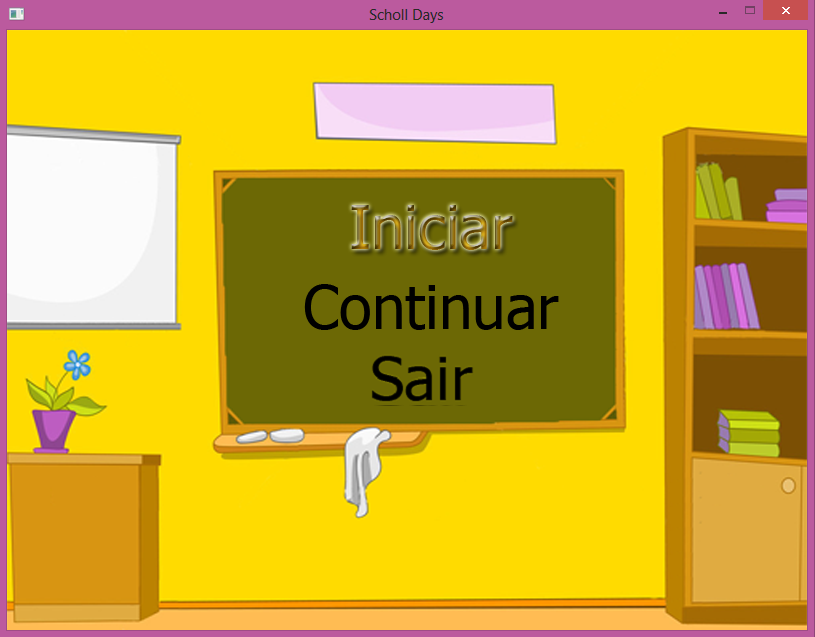
\includegraphics{menu.png}
     \caption{Menu do jogo.}
\end{figure}
\renewcommand{\imsize}{0.3\columnwidth}


\section{Conclusão}

O desenvolvimento do jogo posibilitou uma maior flexibilidade para tratar restrições decorrentes do projeto, tal como o uso da Biblioteca Allegro 5,  e uma abordagem mais crítica sobre um jogo digital não pensando apenas na jogabilidade, mas também na aparência, no enredo e no aprendizado, atraindo assim o público desejado. Mesmo com essas dificuldades o jogo foi finalizando seguindo as propostas e nosso objetivo concluído.
%%% References

%% Note: use of BibTeX als works!!

\bibliographystyle{plain}
\begin{thebibliography}{1}

\bibitem{MATTAR.J}

\newblock {\em MATTAR.J. \bf{Games Em Educação: Como os Nativos Digitais Aprendem}}, São Paulo: Pearson Prentice Hall,2010.

\bibitem{PReNSCKY.M}

\newblock {\em PRENSCKY.M. \bf{Aprendizagem baseada em jogos digitais}}, São Paulo: Senac São Paulo,2012.

\bibitem{TOLEDO.R}

\newblock {\em TOLEDO.R. Tutoriais Allegro 5. Disponível em: http://www.rafaeltoledo.net/tutoriais-allegro-5/}.Último acesso em Novembro de 2013.

\bibitem{Liesenberg}

\newblock {\em Liesenberg. Introdução à Programação em C com Jogos 2D. Disponível em: https://sites.google.com/a/liesenberg.biz/cjogos/home/recursos/allegro-5}.Último acesso em Novembro de 2013

\end{thebibliography}

\end{multicols}

\end{document}

